\chapter{Preprocessing}
\begin{figure}\centering
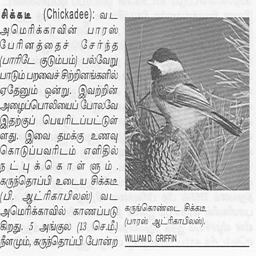
\includegraphics[scale=1]{./img/input}
  \caption{Sample image that is fed to tesseract}\label{INPUT}
\end{figure}
\section{Gray scale conversion}
In grayscale conversion, 24-bit image is converted into 8-bit representation
The input image to be recognised is converted into grayscale using the following formula.
\begin{equation}
I = 0.3R + 0.59G + 0.11B
\end{equation}
where R,G,and B corresponds to red, green and blue intensities respectively.
\begin{figure}\centering

\includegraphics[scale=0.3]{./img/gray}
  \caption{Sample gray scale blob}\label{GRAY}
\end{figure}
\section{Thresholding}
Thresholding refers to the pixel intensity to be used for binarization. For example, if threshold value is 
120, all the pixels having value less than 120 are made zero and the rest as one for binary scale conversion.
\section{Image Binarization}
A binary image is a 2-bit representation of an image. Generally  Otsu's thresholding algorithm 
or sauvola algorithm is used to binarize an image. But it  all depends on the document.
\begin{figure}\centering

\includegraphics[scale=0.3]{./img/bin}
  \caption{Sample binary scale blob}\label{BIN}
\end{figure}
\section{Skew Detection and Correction}
Generally, scanned document has to be skew-corrected because of incorrect orientation of 
document while scanning. There are various algorithms which can be used for skew correction. 
Some of the techniques as given in \cite{praveen} are as follows: projection profile technique , Linear Regression analysis , Fourier Transform based method , nearest neighbor chain , Edge based connected component approach, interline cross-correlation, Entropy based methods. Jonathan J. H. presented a broad survey of existing techniques for skew correction.


\section{Character segmentation}
Character segmentation refers to chopping the words  to individual blobs or characters. It can be carried out by performing connected component analysis\cite{praveen} or ACM based method. 
Before carrying out character segmentation, text level and word level segmentation has to be done.
Generally, the former is done by projection profile technique and the later by k-means clustering\cite{praveen}.
\begin{figure}\centering

\includegraphics[scale=0.3]{./img/junk}
  \caption{Sample of improper segmentation}\label{JUNK}
\end{figure}

\section{Page Layout Analysis}
In page layout analysis, text region is separated from the non-text region and processed. Generally,
voronoi segmentation or RAST based algorithm\cite{amy} is used for layout analysis.
\section{Size Normalization}
Each segmented character is normalized to fit within suitable matrix like 32 x 32 or 64 x 64 so that all characters are of  same size .
\section{Implementation}
We make use of tesseract engine for carrying out the above listed steps. Finally it gives the 
bounding box information from which we extract the corresponding blobs.